\documentclass[aspectratio=169]{beamer}
\usepackage[utf8]{inputenc}
\usepackage[english,russian]{babel}
\usepackage{cancel}
\usepackage{amssymb}
\usepackage{stmaryrd}
\usepackage{cmll}
\usepackage{graphicx}
\usepackage{amsthm}
\usepackage{tikz}
\usepackage{multicol}
\usetikzlibrary{patterns}
\usepackage{chronosys}
\usepackage{proof}
\usepackage{multirow}
\setbeamertemplate{navigation symbols}{}
%\usetheme{Warsaw}

\newtheorem{thm}{Теорема}[section]
\newtheorem{dfn}{Определение}[section]
\newtheorem{lmm}{Лемма}[section]
\newtheorem{exm}{Пример}[section]
\newtheorem{snote}{Пояснение}[section]

\newcommand{\divisible}%
{\mathrel{\lower.2ex%
\vbox{\baselineskip=0.7ex\lineskiplimit=0pt%
\kern6pt \hbox{.}\hbox{.}\hbox{.}}%
}}

\begin{document}

\newcommand\doubleplus{+\kern-1.3ex+\kern0.8ex}
\newcommand\mdoubleplus{\ensuremath{\mathbin{+\mkern-10mu+}}}

\begin{frame}{}
\LARGE\begin{center}Теория множеств\end{center}
\end{frame}

\begin{frame}{Теория множеств}
\begin{enumerate}
\item Георг Кантор: 1877 год, <<наивная теория множеств>>. Множество --- это «объединение в одно
целое объектов, хорошо различаемых нашей интуицией или нашей мыслью».\pause
\item Неограниченный принцип абстракции $\{ x\ |\ P(x)\}$ \pause
\item Парадокс Бурали-Форти (1895, Кантор). Парадокс Рассела: $X := \{ x\ |\ x \notin x\}$; $X\in X$?\pause
\item Вариант решения парадокса: а, может, запретить все <<опасные>> ситуации? \pause
\item Аксиоматика Цермело --- 1908 год, оставим только то, что используют математики. \pause
\item Что такое множество? Неформально мы понимаем, формально:\pause

\begin{dfn} Теория множеств --- теория первого порядка,
с дополнительным нелогическим двухместным функциональным символом $\in$, и следующими 
дополнительными нелогическими аксиомами и схемами аксиом.
\end{dfn}
\end{enumerate}
\end{frame}

\begin{frame}{Аксиоматика ZF, равенство}
\begin{dfn} Равенство <<по Лейбницу>>: объекты равны, если неразличимы.\end{dfn} Если нечто ходит как утка, выглядит как 
утка и крякает как утка, то это утка.\pause
\begin{dfn} Принцип объёмности: объекты равны, если состоят из одинаковых частей\end{dfn}\pause

\begin{dfn} $A \subseteq B \equiv \forall x.x \in A \rightarrow x \in B$ \\\pause
 $A = B \equiv A \subseteq B \with B \subseteq A$ \end{dfn}\pause
\begin{dfn} Аксиома равенства: равные множества содержатся в одних и тех же множествах. 
$\forall x. \forall y. \forall z. x = y \with x \in z \rightarrow y \in z$.
\end{dfn}
\end{frame}

\begin{frame}{Аксиоматика ZF, конструктивные аксиомы}
\begin{dfn} Аксиома пустого. Существует пустое множество $\varnothing$. $$\exists s.\forall t.\neg t \in s$$ \end{dfn}\pause
\begin{dfn} Аксиома пары. Существует $\{a,b\}$.
Каковы бы ни были два множества $a$ и $b$, существует множество, состоящее 
в точности из них. 

$$\forall a.\forall b.\exists s.a \in s \with b \in s \with \forall c.c \in s \rightarrow c = a \vee c = b$$ \end{dfn}
\end{frame}

\begin{frame}{Аксиоматика ZF, конструктивные аксиомы 2}
\begin{dfn} Аксиома объединения: существует $\cup x$. 
Для любого непустого множества $x$ найдется такое множество, состоящее в точности
из тех элементов, из которых состоят элементы $x$. 
$$\forall x.(\exists y.y \in x) \rightarrow \exists p.\forall y.y \in p \leftrightarrow \exists s.y \in s \with s \in x$$
 \end{dfn}\pause
\begin{dfn} Аксиома степени: существует $\mathcal{P}(x)$.
Каково бы ни было множество $x$, существует множество, содержащее в точности
все возможные подмножества множества $x$.
$$\forall x.\exists p.\forall y.y \in p \leftrightarrow y \subseteq x$$
\end{dfn}
\end{frame}

\begin{frame}{Аксиоматика ZF. Схема аксиом выделения}
\begin{dfn} Схема аксиом выделения: существует $\{ t \in x\ |\ \varphi(t)\}$.
Для любого множества $x$ и любой формулы от одного аргумента $\varphi(y)$
($b$ не входит свободно в $\varphi$), найдется $b$, в которое
входят те и только те элементы из множества $x$, что $\varphi(y)$ истинно.

$$\forall x.\exists b.\forall y.y \in b \leftrightarrow (y \in x \with \varphi(y))$$
\end{dfn}
\end{frame}

\begin{frame}{Немного теорем}
\begin{thm}Для любого множества $X$ существует множество $\{X\}$, содержащее в точности $X$.\end{thm}\pause
\begin{proof}Воспользуемся аксиомой пары: $\{X,X\}$\end{proof}\pause
\begin{thm}Пустое множество единственно.\end{thm}\pause
\begin{proof}Пусть $\forall p.\neg p \in s$ и $\forall p.\neg p \in t$.
Тогда $s \subseteq t$ и $t \subseteq s$.\end{proof}\pause
\begin{thm}Для двух множеств $s$ и $t$ существует множество, являющееся их пересечением.\end{thm}\pause
\begin{proof}$s \cap t = \{ x\in s\ |\ x \in t\}$\end{proof}
\end{frame}

\begin{frame}{Упорядоченная пара}
\begin{dfn}{Упорядоченная пара.}
Упорядоченной парой двух множеств $a$ и $b$ назовём
$\{\{a\},\{a,b\}\}$, или $\langle{}a,b\rangle$
\end{dfn}

\begin{thm}
Упорядоченную пару можно построить для любых множеств.
\end{thm}
\begin{proof}Применить аксиому пары, теорему о существовании $\{X\}$, аксиому пары.\end{proof}

\begin{thm}
$\langle{}a,b\rangle = \langle{}c,d\rangle$ тогда и только тогда,
когда $a = c$ и $b = d$.
\end{thm}
\end{frame}

\begin{frame}{Аксиома бесконечности}
\begin{dfn}Инкремент: $x' \equiv x \cup \{x\}$\end{dfn}\pause
\begin{dfn}Аксиома бесконечности. Существует $N: \varnothing \in N \with \forall x.x \in N\rightarrow x' \in N$\end{dfn}\pause

В $N$ есть всевозможные множества вида $\varnothing$\pause, $\{\varnothing\}$\pause, $\{\varnothing,\{\varnothing\}\}$, \pause
$\{\varnothing,\{\varnothing\},\{\varnothing,\{\varnothing\}\}\}$, \dots\pause
\\\vspace{0.5cm}
(неформально) $\omega = \{\varnothing, \varnothing', \varnothing'', \dots\}$. \pause
Тогда $N_1 = \omega\cup\{\omega,\omega',\omega'',\dots\}$ подходит.
\end{frame}

\begin{frame}{Полный порядок (вполне упорядоченные множества)}
\begin{enumerate}
\item Частичный: рефлексивность ($a \preceq a$), антисимметричность ($a \preceq b \rightarrow b \preceq a\rightarrow a=b$),
транзитивность ($a \preceq b \rightarrow b \preceq c \rightarrow a \preceq c$).\pause
\item Линейный: частичный + $\forall a.\forall b.a \preceq b \vee b \preceq a$.\pause
\item Полный: линейный + в любом непустом подмножестве есть наименьший элемент.\pause
\end{enumerate}

\begin{exm}$\mathbb{Z}$ не вполне упорядочено: в $\mathbb{Z}$ нет наименьшего.\end{exm}\pause
\begin{exm}Отрезок $[0,1]$ не вполне упорядочен: $(0,1)$ не имеет наименьшего.\end{exm}\pause
\begin{exm}$\mathbb{N}$ вполне упорядочено.\end{exm}
\end{frame}

\begin{frame}{Ординалы (порядковые числа)}
\begin{dfn}Транзитивное множество $X$: $\forall x.\forall y.x \in y \with y \in X \rightarrow x \in X$.\end{dfn}\pause
\begin{dfn}Ординал (порядковое число) --- вполне упорядоченное отношением $(\in)$ транзитивное множество.\end{dfn}\pause
\begin{exm}Ординалы: $\varnothing$, \pause $\varnothing'$, \pause $\varnothing''$, \dots\end{exm}\pause
\begin{dfn}Предельный ординал: такой $x$, что $x \ne \varnothing$ и нет $y: y' = x$\end{dfn}\pause
\begin{dfn}Ординал $x$ конечный, если он сам не предельный и нет предельного, меньшего его.\end{dfn}\pause
\begin{thm}Если $x,y$ --- ординалы, то $x = y$, или $x\in y$, или $y \in x$.\end{thm}
\end{frame}
\begin{frame}{Предельные ординалы, $\omega$}
\begin{dfn}$\omega$ --- наименьший предельный ординал.\end{dfn}\pause
\begin{thm}$\omega$ существует.\end{thm}\pause
\begin{proof}Пусть $\omega = \{ x \in N\ |\ x\text{ конечен}\}$. Тогда:
\begin{itemize}
\item меньше $\omega$ предельных нет: если $\theta$ таков, что $\theta \in \omega$, тогда $\theta$ конечен.\pause
\item $\omega$ предельный: Пусть $\theta$ таков, что $\theta' = \omega$. Тогда $\theta$ конечен и $\theta'$ тоже конечен.
\end{itemize}\end{proof}
\begin{exm}$\omega'$ --- тоже ординал.\end{exm}
\end{frame}

\begin{frame}{Порядковый тип}
\begin{dfn}[неформальное определение]Порядковый тип множества --- некоторое свойство, общее для всех множеств, 
изоморфных относительно биективных отображений, сохраняющих порядок.\end{dfn}

\begin{dfn}Порядковый тип вполне упорядоченного множества $\langle S, (\preceq)\rangle$ --- ординал $A$, для которого есть биективное отображение $f: S \rightarrow A$, сохраняющее порядок:
$a \preceq b$ тогда и только тогда, когда $f(a) \le f(b)$\end{dfn}

\begin{exm}Множество $\mathbb{Z}$ не имеет порядкового типа (в смысле определения через ординалы): оно не вполне упорядочено.\end{exm}
\end{frame}

\begin{frame}{Операции над ординалами}
\begin{dfn}$a + b$ --- порядковый тип $a \uplus b$ (отмеченного объединения), причём $x_a < y_b$ при любых
$x \in a$ и $y \in b$\end{dfn}

\begin{dfn}$a \cdot b$ --- порядковый тип $a \times b$, произведение упорядочено лексикографически: $\langle x_1, y_1 \rangle < \langle x_2, y_2 \rangle$, 
если $x_1 < x_2$ или $x_1 = x_2$ и $y_1 < y_2$.\end{dfn}

\begin{exm}$\overline{3} + \overline{4}$: порядковый тип множества $\{0_a, 1_a, 2_a, 0_b, 1_b, 2_b, 3_b\}$, то есть $\overline{7}$

$\overline{\omega} \cdot \overline{\omega}$: порядковый тип всех натуральных точек плоскости, $\{\langle 0,0 \rangle, \dots, \langle 0,100\rangle, \dots, \langle 100,0\rangle, \dots\}$\end{exm}
\end{frame}

\begin{frame}{Операции над ординалами --- как вычислять}
\begin{dfn}$\text{upb } x$ --- верхняя грань множества ординалов, $\text{upb }x = \bigcup_{a \in x} a$.\end{dfn} \pause
\begin{exm}$\text{upb } \{ \varnothing', \varnothing'', \varnothing'''' \} = \varnothing' \cup \varnothing'' \cup \varnothing'''' =
\{ \varnothing \} \cup \{ \varnothing, \{ \varnothing \} \} \cup \{ \varnothing, \{ \varnothing \}, \{ \varnothing, \{ \varnothing \} \}, \{ \varnothing, \{ \varnothing \}, \{ \varnothing, \{ \varnothing \} \} \} \}
= \pause \varnothing''''$\end{exm} \pause

\begin{thm}
$$a + b \equiv \left\{ \begin{array}{rl} 
   a, & b \equiv \varnothing\\
   (a + c)', & b \equiv c'\\
   \text{upb } \{ a+c \mid c \prec b \}, &\mbox{$b$ --- предельный ординал }\end{array}\right.$$\end{thm}

\begin{exm}$\omega + 1 = \omega \cup \{\omega\}$; \pause $1 + \omega = \text{upb }\{ 1+\varnothing, 1+1, 1+2, \dots \} \pause = \omega$\end{exm}
\end{frame}

\begin{frame}{Ещё операции над ординалами}
\begin{thm}
$$a \cdot b \equiv \left\{ \begin{array}{rl} 
   0, & b \equiv \varnothing\\
   (a \cdot c) + a, & b \equiv c'\\
   \text{upb } \{ a \cdot c \mid c \prec b \}, &\mbox{$b$ --- предельный ординал }\end{array}\right.$$
\end{thm}
\pause
\begin{dfn}
$$a ^ b \equiv \left\{ \begin{array}{rl} 
   1, & b \equiv \varnothing\\
   (a ^ c) \cdot a, & b \equiv c'\\
   \text{upb } \{ a^c \mid c \prec b \}, &\mbox{$b$ --- предельный ординал }\end{array}\right.$$
\end{dfn}
\pause
\begin{exm}$\omega \cdot \omega = \text{upb }\{\omega \cdot 0, \omega \cdot 1,\omega\cdot 2, \omega\cdot 3, \dots\} = \text{upb }\{0, \omega,\omega\cdot 2, \omega\cdot 3, \dots\}$\end{exm}
\end{frame}

\begin{frame}{Ординалы (порядковые числа) и порядок}
\begin{exm}\begin{itemize}
\item Добавить элемент перед бесконечностью: $\mathbb{N}$ и $\mathbb{N}_0$.
\pause
$1 + \omega = \omega$. \pause
\item Добавить элемент после бесконечности $(+\infty)$. \pause $\omega + 1 \ne \omega$ \pause
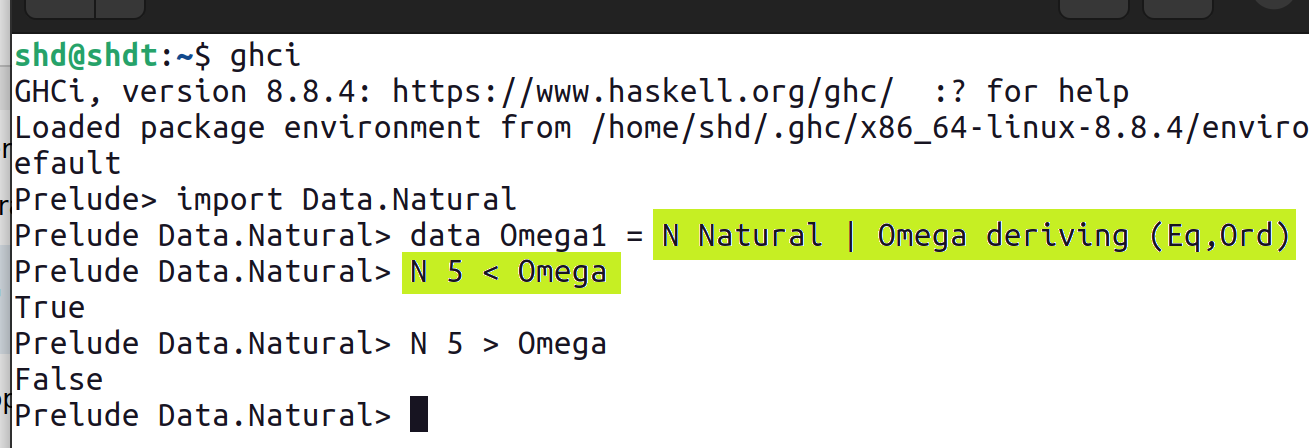
\includegraphics[scale=0.9]{pics/lection-13-ghc}
\end{itemize}\end{exm} 
\end{frame}

\begin{frame}{Пары и списки}
\begin{exm}Упорядоченные пары натуральных чисел имеют порядковый тип $\omega^2$.\pause

\begin{center}$\langle 3,5 \rangle < \langle 4,3 \rangle\quad\quad\omega \cdot 3 + 5 < \omega \cdot 4 + 3$.\end{center}\end{exm}\pause

\begin{exm}Списки натуральных чисел --- порядковый тип $\omega^\omega$.
$$\langle 3,1,4,1,5,9\rangle\quad\quad \omega^5 \cdot 3 + \omega^4 \cdot 1 + \omega^3 \cdot 4 + \omega^2 \cdot 1 + \omega^1 \cdot 5 + 9$$\end{exm}
\end{frame}

\begin{frame}{Дизъюнктные множества}
\begin{dfn}Дизъюнктное (разделённое) множество --- множество, элементы которого
не пересекаются. 
$$Dj(x) \equiv \forall y.\forall z.(y \in x \with z \in x \with \neg y=z) \rightarrow 
\neg \exists t.t \in y \with t \in z$$
\end{dfn}\pause

\begin{exm}Дизъюнктное: $\{\{1,2\},\{\rightarrow\},\{\alpha,\beta,\gamma\}\}$\\ \pause
Не дизъюнктное: $\{\{1,2\},\{\rightarrow\},\{\alpha,\beta,\gamma,1\}\}$
\end{exm}
\end{frame}

\begin{frame}{Прямое произведение множеств}
\begin{dfn}Прямое произведение дизъюнктного множества $a$ --- 
множество $\times a$ всех таких множеств $b$, что:
\begin{itemize}
\item $b$ пересекается с каждым из элементов множества $a$ в точности в одном элементе
\item $b$ содержит элементы только из $\cup a$.
\end{itemize}

$$\forall b .b \in \times a \leftrightarrow (b \subseteq \cup a \with \forall y .y \in a \rightarrow \exists ! x .x \in y \with x \in b)$$
\end{dfn}\pause

\begin{exm}
$\times\{\{\triangle,\square\},\{1,2,3\}\} = \{\{\triangle,1\},\{\triangle,2\},\{\triangle,3\},\{\square,1\},\{\square,2\},\{\square,3\}\}$
\end{exm}

\end{frame}

\begin{frame}{Аксиома выбора}
\begin{dfn}
Прямое произведение непустого дизъюнктного множества, 
не содержащего пустых элементов, непусто.

$$\forall t.Dj (t) \rightarrow 
(\forall x.x \in t \rightarrow \exists p.p \in x) \rightarrow
(\exists p.p \in \times t)$$
\end{dfn}\pause

Альтернативные варианты: любое множество можно вполне упорядочить, \pause любая сюръективная функция имеет частичную обратную, 
и т.п.
\begin{dfn}Аксиоматика ZF + аксиома выбора = ZFC\end{dfn}\pause
\end{frame}

\begin{frame}{Дискуссия вокруг аксиомы выбора}
\begin{exm}Парадокс Банаха-Тарского: трёхмерный шар равносоставен двум своим копиям.\end{exm}\pause
\begin{thm}Теорема (Гёдель, 1938): аксиома выбора не добавляет противоречий в ZF.\end{thm}\pause
\begin{thm}Теорема (Коэн, 1963): аксиома выбора не следует из других аксиом ZF.\end{thm}\pause
\begin{exm}Односторонние функции: Sha256 и т.п. У Sha256 есть обратная.\end{exm}\pause
\begin{thm}Теорема Диаконеску: ZFC поверх интуиционистского исчисления предикатов содержит правило исключённого третьего.\end{thm}
\end{frame}

\begin{frame}{Аксиома фундирования}
\begin{dfn}Аксиома фундирования. 
В каждом непустом множестве найдется элемент, не пересекающийся с исходным множеством.
$$\forall x .x = \varnothing \vee \exists y .y \in x \with \forall z.z \in x \rightarrow z \notin y$$
\end{dfn}

Иными словами, в каждом множестве есть элемент, минимальный по отношению $(\in)$.

Идея Рассела: каждому множеству припишем \emph{тип} (тип пустого 0, тип множеств 1,
тип множеств множеств 2 и т.п.). Тогда конструкция невозможна: $\{ x\ |\ x \in x\}$.
Аксиома фундирования позволяет определить функцию ранга:
$$rk(x) = \text{upb }\{rk(y)\ |\ y\in x\}$$.
\end{frame}

\begin{frame}{Схема аксиом подстановки}
\begin{dfn}Схема аксиом подстановки. 
Пусть задана некоторая функция f, представимая в исчислении предикатов:
то есть задана некоторая формула $\phi$, такая, что $f(x) = y$
тогда и только тогда, когда $\phi(x,y) \with \exists ! z. \phi(x,z)$.
Тогда для любого множества S существует множество f(S) --- образ
множества S при отображении f.
$$\forall s .(\forall x .\forall y_1 .\forall y_2 .x \in s \with \phi (x,y_1) \with \phi
(x,y_2) \rightarrow y_1=y_2) \rightarrow 
(\exists t .\forall y .y \in t
\leftrightarrow \exists x . x \in s \with \phi (x,y)) $$
\end{dfn}
\end{frame}

\end{document}
